\icode{E-MD-SI-L2-261114-011}
如图所示，球壳内有三条弦 \(OA\)、\(OB\)、\(OC\)，\(O\) 为球内的最低点，它们与水平面间的夹角分别为\qty{60}{\degree}、\qty{45}{\degree}、\qty{30}{\degree}。三个光滑的小环分别从 \(A\)、\(B\)、\(C\) 处由静止沿所在弦下滑，运动到最低点所用的时间分别为 \(t_A\)、\(t_B\)、\(t_C\)，则三者之间大小关系为\paren[]
	
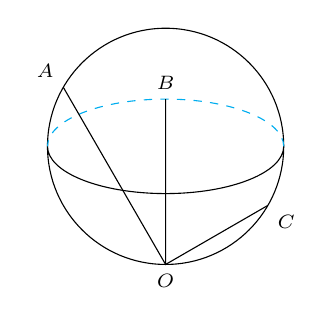
\begin{tikzpicture}[font=\scriptsize]
	\draw (0,0) circle(1.5) (-1.5,0) arc(-180:0:1.5 and .6);
	\draw[dashed,cyan] (1.5,0) arc(0:180:1.5 and .6);
	\draw (150:1.5)node[above left]{\(A\)}--(0,-1.5)node[below]{\(O\)}--(-30:1.5)node[below right]{\(C\)} (0,-1.5)--(0,.6)node[above]{\(B\)};
\end{tikzpicture}
\begin{choices}
	\item \(t_A = t_B = t_C\)
	\item \(t_A < t_B < t_C\)
	\item \(t_A > t_B > t_C\)
	\item \(t_A = t_C > t_B\)
\end{choices}
\begin{answer}
    A\qquad 提示：
\end{answer}